\documentclass[a4paper,10pt]{IEEEconf}
\usepackage[latin1]{inputenc}
\usepackage[american]{babel}
%\usepackage[T1]{fontenc}
\usepackage[dvips,pdftex]{graphicx}
%\usepackage{multicol}
\usepackage{subfigure}
\usepackage{named}
%\usepackage{fancybox}
%\usepackage{natbib}
\bibliographystyle{named}
\usepackage[dvips,pdftex]{hyperref}
%opening
\title{ Symbol Recognition using Particle Swarm Algorithms}
%\title{A Study on Using Particle Swarm Algorithms in Symbol Recognition }
\author{Maha El Meseery, Dr. Mahmoud Fakhr El Din, Dr. Samyah Mashaly,
\\ Dr. Magdah Fayek, Dr. Nevin Darwish}
\begin{document}
\maketitle
\begin{abstract}
Sketch recognition is defined by the process of identifying the symbols the user draws using a single or multiple strokes. Users draw strokes using a pen and the system immediately interprets their strokes into objects that can be easily manipulated. This paper uses Particle Swarm Algorithm(PSO) to divide strokes a user draws into meaningful geometric primitives. These geometric primitives are grouped to formulate symbols which will be further identified. The results showed that using PSO improves segmentation results which guide the symbol recognition phase. Final recognition have improved after the PSO algorithm using a SVM classifier.  
 %Hand drawn sketches are the natural method of exchanging thoughts between engineers and humans in general. Nevertheless, researchers barely give attention to improve current gesture and sketch recognition systems. In a sketch understanding system, users need to feel the freedom of paper and pencil along with the flexibility of computer manipulation. 
\end{abstract}
\section{Introduction}
%A picture speak a thousand words is also true for sketches. 
Scientists in general and engineers specifically express thoughts and designs using sketches. Engineers use sketches to exchange designs as a natural method of communication rather than writing or speaking. Currently, engineers use paper and pencil design in early stages of design. Design engineers need a powerful symbol recognition and manipulation system to help them operate as freely as with papers. Increasing the interaction between the computer and the users in sketch and CAD systems was recently the reason for the emerging of few advanced sketch recognition systems. Sketch recognition system converts the drawings and informal graphs the user draws into objects and symbols can be used in further interaction with the system. \\
Most researchers in sketch recognition divided the system into four main steps preprocessing, segmentation, symbol recognition and finally sketch understanding. The preprocessing process saves the location of points from the hardware and collects basic information about the stroke data. After removing noise and calculating primary data the system proceeds to divide the stroke into a set of simple geometrical primitives.  The second step of the system is clustering strokes and segments to formulate symbols that can be recognized by the system. Finally, priori information about the sketch is used to support identification of symbols by excluding any possible invalid symbols. \\
%the basic symbols are identified in consistent with the whole sketch. \\
%from the user information from the users converts the strokes the user draw into segments which is recognized into basic symbols that can be easily manipulated. Finally, the basic symbols are interpreted in consistent with the whole sketch. \\
The next section will relate previous work in the field. The remaining of the paper will be as following; Section \ref{PSO} will explain the general particle swarm algorithm. Section \ref{Sysdisc} will describe the system block diagram and then section \ref{Prepross} will explain the preprocessing step, section \ref{seg} will describe the segmentation algorithm in details. Finally, section \ref{sec:Experiments} will describe the experiments that was preformed.\\
\section{Related Work}
%%%What is sketch recognitions. Why we need sketch recognition systems. 
The field of symbol recognition has gained interest in the last few years. A wide variety of techniques were used either on segmentation process or symbol recognition.\\ 
To segment strokes, \cite{meanshift10} introduced a feature area for each primitive and then compute the segmentation error for different types of primitives based on this area. %\citeauthor{HeloiseBeautification} used a dynamic programming algorithm to solve the segmentation problem \cite{HeloiseBeautification}. 
Complex and hybrid algorithm were also introduced as in  \cite{earlyprocess} where they generated different sets of segmentation based on both curvature and speed dominant points then they choose the segmentation with the least error from the hybrid set. A dynamic programming algorithm was also used to obtain optimum segmentation of the input strokes in \cite{GeometryAndDomain102}. Genetic algorithm was also used by \cite{CruveDivisionSwarm} to optimally divide digital curves into lines and curves. \cite{PolygonApproximationPSO} used PSO to convert digital curves into polygons.  \\
  %Some tried to detect dominant or corner points based on data generated from speed   \cite{earlyprocess} and mostly used curvature of the stroke drawn \cite{earlyprocess,meanshift10}. 

%Particle swarm algorithms was used in \cite{} to fit a set of points into ellipse or higher order curves.
%The first set of features introduced to be used on gesture recognition was introduced by Rubine in \cite{gestureexample12}. later,  Spatial relations and features where used in  \cite{cognitivesketch18,SRGraph57}  . \citeauthor{GeometryAndDomain102} introduced ink density feature which they used.  The use of Zernike moments  was used  as the only features to the SVM classifiers in \cite{HeloiseBeautification}.  \cite{SketchRead2007} used a set of features varied from relative spatial features and some compositional features.  \\

%After segmentation researchers varies on the methods in which to continue.
Many different approaches have been investigated to achieve final recognition of symbols. Graph searching and template matching where used in \cite{mulitstroke5,GraphBased07}, where  a graph of the drawn symbol is generated and matched to stored set of graphs templates to reach a classification. Geometrical and spatial descriptive language was used in \cite{SketchRead2007,Ladder30} where a parser like architecture was used to recognize symbols  . \citeauthor{imagetrainable48} used trainable image template to classify different set of symbols \cite{imagetrainable48} .  The use of SVM and HMM classification was implemented in \cite{SVM300,SmartSketch56} and \cite{HMM53}.\\% Other techniques as  [          ] was used  in []. \\  
 %In the next section the particle swarm algorithm will be explained. After that the system block description and detailed algorithms will be described. We will then proceed to describe the experiments preformed and the achieved results.  
%\subsection{Sketch Recognitions systems}
%Details of Sketch systems. 
%Related work and research in this area. 
%Writing on the pros and cons of current systems.  
%Write on the difficulties of the sketch recognition systems. 
\subsection{Particle Swarm Algorithm}
\label{PSO}
%What is particle swarm algorithm and how it was used in related researches. 
In the Particle Swarm Algorithm (PSO) each agent represents a particle from the solution space. The agents move the particle with direction and velocity based on the general swarm equation [\ref{eq:Swarm}]. Equation [\ref{eq:Swarm}] shows how velocity and direction of each particle is computed where $r_1$ \& $r_2$ are random variable and $c_1$ \& $c_2$ are the swarm system variables. Each iteration the global best $g_{best}$ particle and  the agent local best $l_{best}$ particle are evaluated based on the maximum fitness functions of  all particles. The solution is found after a maximum number of iteration or after an error threshold is achieved. Equation \ref{eq:descrite} where t is a threshold and $r_{3}$  is a random variable, is used to change general swarm algorithm into binary particle which will handle particle values of either 0 or 1. .  
\begin{equation}
%\[
v_{ij}  = v_{ij}  + c_1 r_1 (lbest_{ij}  - p_{ij} ) + c_2 r_2 (gbest_{ij}  - p_{ij} )
%\]
\label{eq:Swarm}
\end{equation}
\begin{equation}
%\[
p_{ij}=p_{ij}+v_{ij},
%\]
\end{equation}
\begin{equation}
   P(i)\Leftarrow 
\{
\begin{array}{c} 
1 \quad \quad if\quad r_{3}>t  \\

0 \quad \quad if\quad r_{3}<t 
\label{eq:descrite}
\end{array}\}
\end{equation}
\section{System Description}
\label{Sysdisc}
%The stroke is the path of points from the instant the pen is down till it is up.
As shown in fig. \ref{fig:Blockdiagram} the system is divided into four main blocks. Preprocessing, segmentation, clustering, feature extraction and finally classification. \\
 %Due to sloppiness of users and hardware glitches the system preprocesses the data before further processing. 
 The preprocessing block is responsible of capturing the input data and removing the noise from it. The system then proceeds to estimate a set of possible dominant points to help in the segmentation process.  \\% The time differences, direction, speed and curvature of all points of the stroke is computed along with some other geometrical data. The system then proceed to estimate a set of possible dominant points to help in segmentation process.  \\
  %then passes through the segmentation process which will try to 
 %The goal of the segmentation stage is to divide stroke into segments of either curves or lines.
  The segmentation process is divided into two steps ellipse fitting and  curve segmentation. In the first step, the system tries to fit the stroke into an ellipse. If the system fails it passes the stroke into two PSO segmentation algorithms. The two algorithms will generate two segmentations, the system will choose the segmentation that has the minimum segmentation error.%  generate the segmentations,  the minimum error will be the chosen segmentation. % is the ellipse fitting
 %the stroke first If the ellipse detection fails the stroke is passed to the segmentation algorithms which will pass it to the two PSO algorithms described below the segmentation with the minimum error will be the chosen segmentation.  The segmentation is then added to the set of un-recognized segments in the system. \\% This part is repeated for each stroke. 
 
After the user finish sketching the symbol by using any number of strokes, the set of unrecognized segments is passed to the feature extraction and classifier.% The system compute composite set of features some are statistical other are spatial features based on the type primitives. Finally, the strokes are classified into the corresponding classes.% the classifier identifies the strokes into a symbol from the set of known symbols.\\
\begin{figure}[]
	\centering
		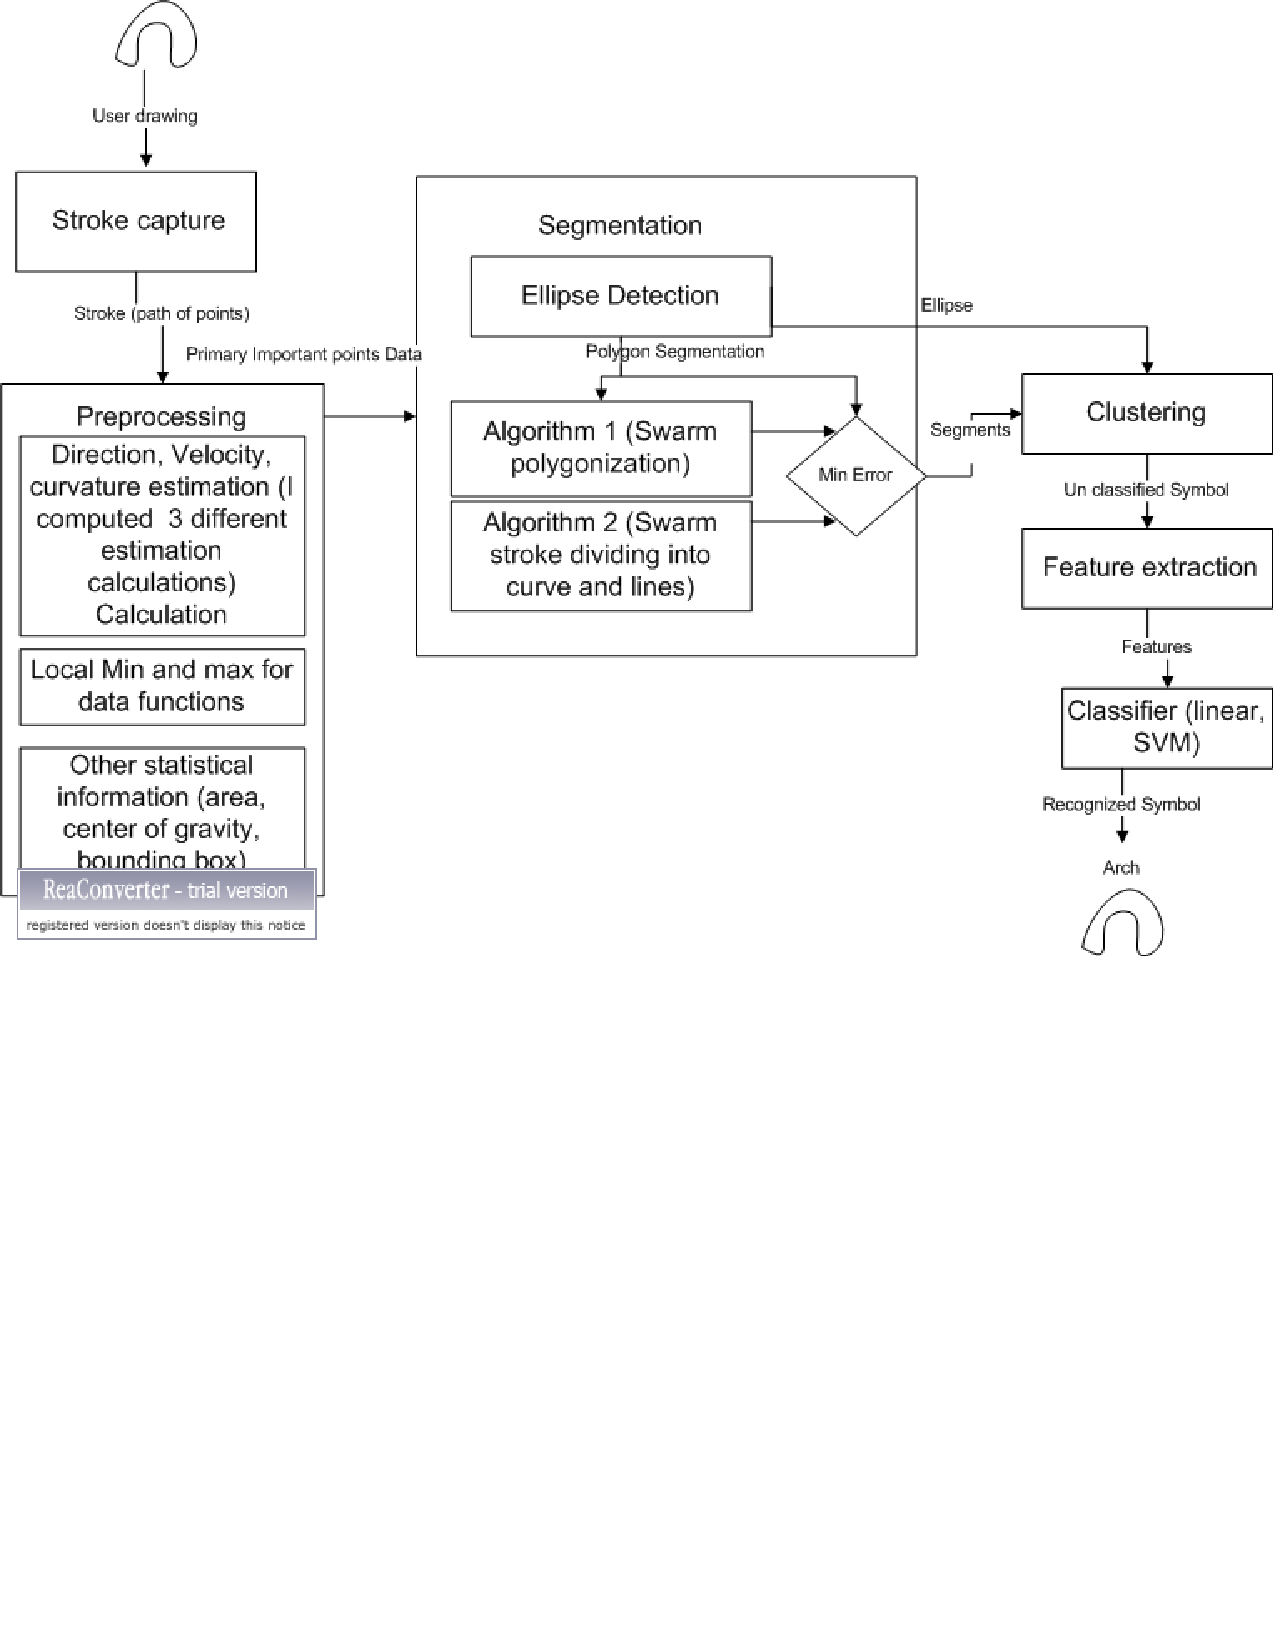
\includegraphics[scale=0.35]{images/Blockdiagram.pdf}
	\caption[  ]{The system Block Diagram}
	\label{fig:Blockdiagram}
\end{figure}
\subsection{Preprocessing}
\label{Prepross}
%Some data is extracted from the points in the stroke.
 It was noted that as the user draws a shape the pen will slow down near corners and will pick up speed when drawing a straight lines. Therefore, the speed and time difference data were widely used in sketch understanding systems \cite{earlyprocess}.  The direction and curvature data are used to decide the points with high angular changes along the path of points\cite{meanshift10}.  \\
 
 In the presented system, we computed time difference, direction, speed and curvature of each point along the stroke. For speed calculation $v=\Delta t/\Delta s$ where t is the time difference between two points and s is the length between them. The direction is calculated as the angle between two vectors and curvature is the change in direction with respect to length i.e. $c= \Delta d/\Delta s$. \\
 %system compute speed, distance data for all points in the stroke. Curvature is computed using estimation used in [] where direction computed is angle between two lines. Curvature is 
 %$\Delta d/  \Delta S $ where d is the difference direction of point and s is difference in distance between points. 
 All the calculations are performed in real time while the user draws his strokes.
 So the resultant computation complexity of computing of all these computation is O(n) where n is number of points. \\
 Figure \ref{fig:speed2} shows the computed data for the stroke drawn in fig. \ref{fig:orignalStroke}.  If you look at the data curves you will see that dominant points are characterized by lower speed values and higher curvature and direction values. \\% the lower speed points correspond to vertex and dominant point's location. The higher the direction and curvature data correspond to location with higher change in curvature witch promote the location for vertices. \\
After the system computes all the speed, time difference and curvature data it proceeds to detect the points with low velocity and high curvatures. Using simple differentiations to detect local extreme points resulted in false points due to the non smooth curves. So instead the following procedure was used, firstly the mean of the curve is used as threshold for lower values then the high values are further investigated to find the extreme points. Hence, the mean of the direction curve is calculated and used as threshold. This threshold is used to separate the curve into regions; each region is defined as the part between two intersection points of the threshold line and the curve. Only regions higher than the threshold value are processed when computing the maximum of each region. The point that corresponds to those maximum values are labeled possible dominant points.   \\
   %If we tried to differentiate the curve the result will be false threshold values we divide the data into regions of data higher or lower that the threshold. This will let us only look for high data only. The maximum of each region is then computed and reported as a possible vertex point. 
\begin{figure}[]
	\centering
		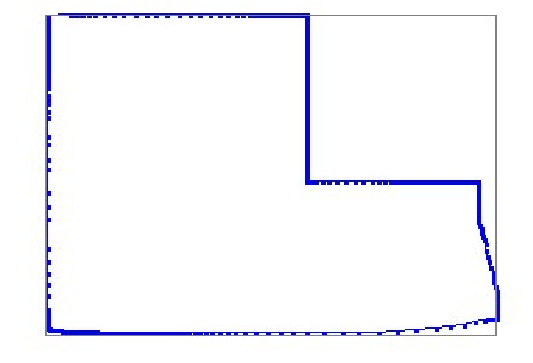
\includegraphics[scale=0.3]{images/orignalStroke.pdf}
	\caption{Stroke Sample}
	\label{fig:orignalStroke}
\end{figure}
The system repeat this process to curvature, time difference and speed curves. All the points labeled as possible dominant points are saved into a single array. They are used as input and guiding data for the next stage of segmentation. 
\begin{figure*}[]
\begin{minipage}[b]{0.5\linewidth}
	\centering

		\subfigure[ The Speed of data] {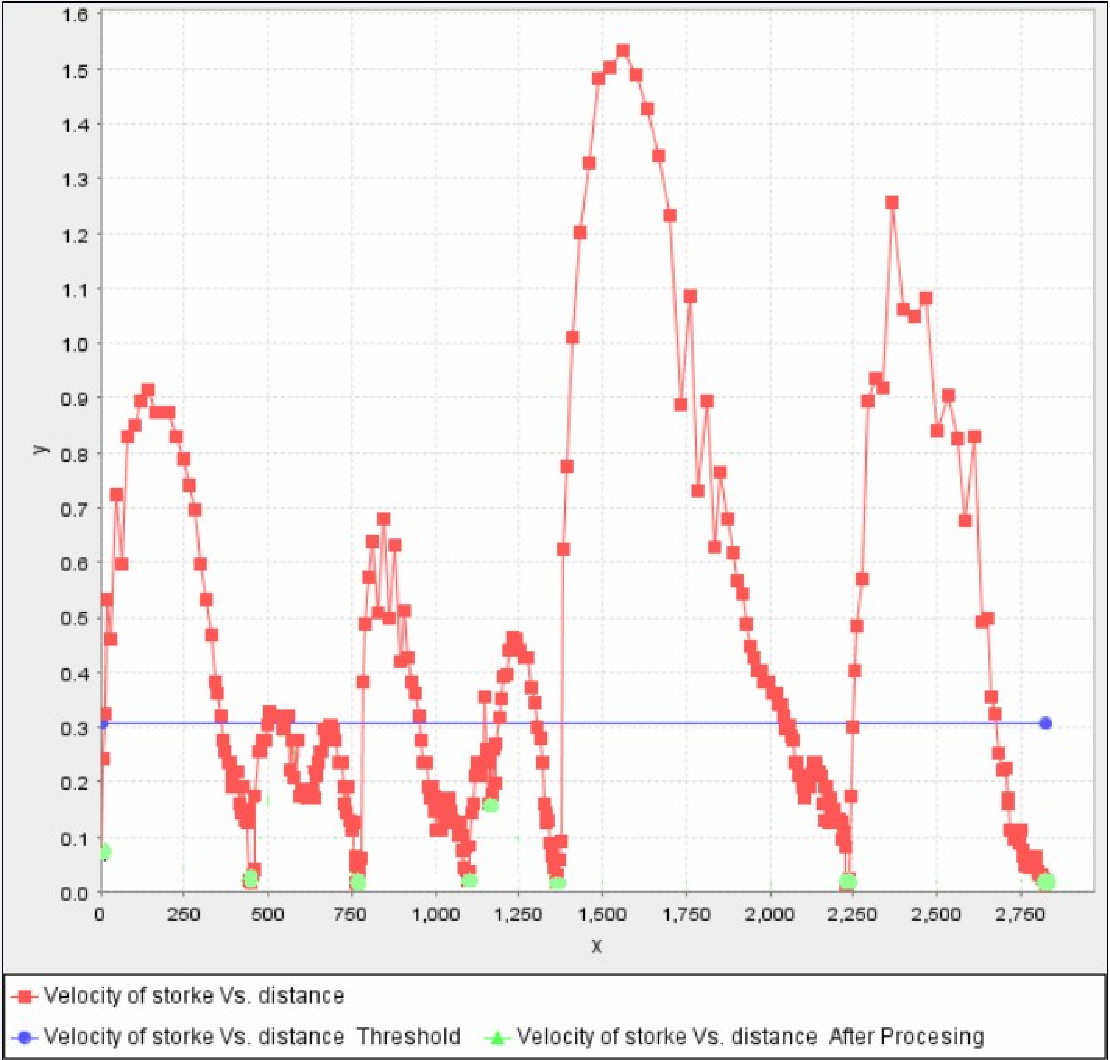
\includegraphics[scale=0.15]{images/speed2.pdf}}
		
		\subfigure[ Direction ] {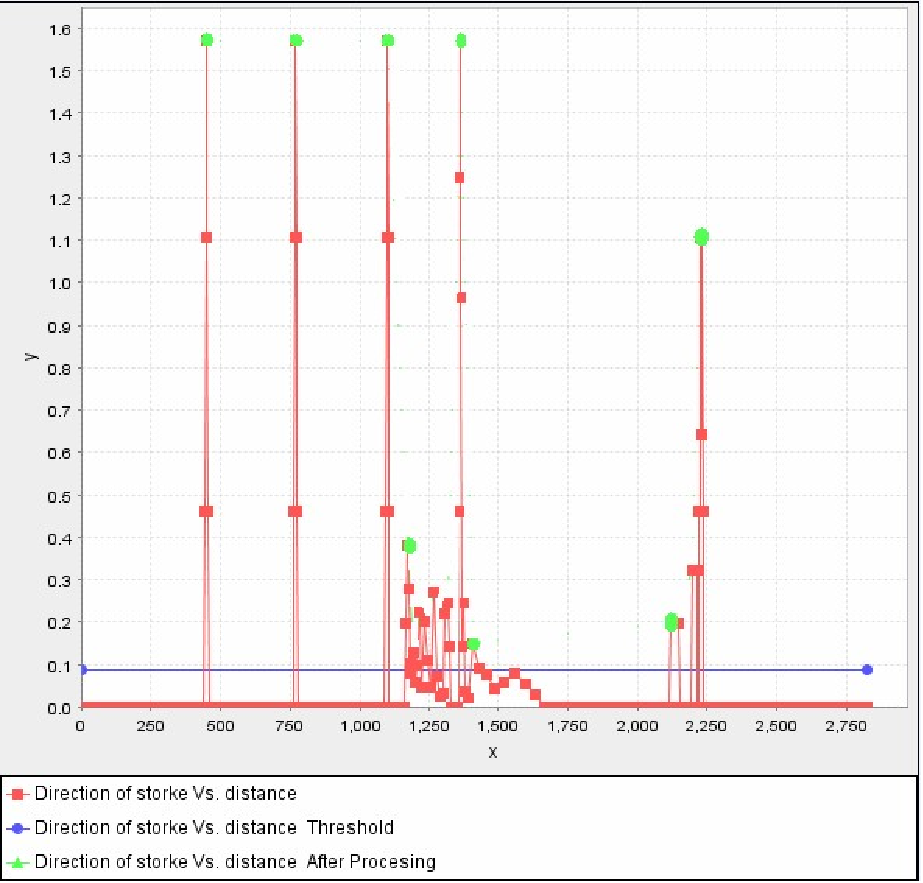
\includegraphics[scale=0.15]{images/direction2.pdf}}
					\end{minipage}
					\begin{minipage}[b]{0.5\linewidth}
			\subfigure[Curvature] {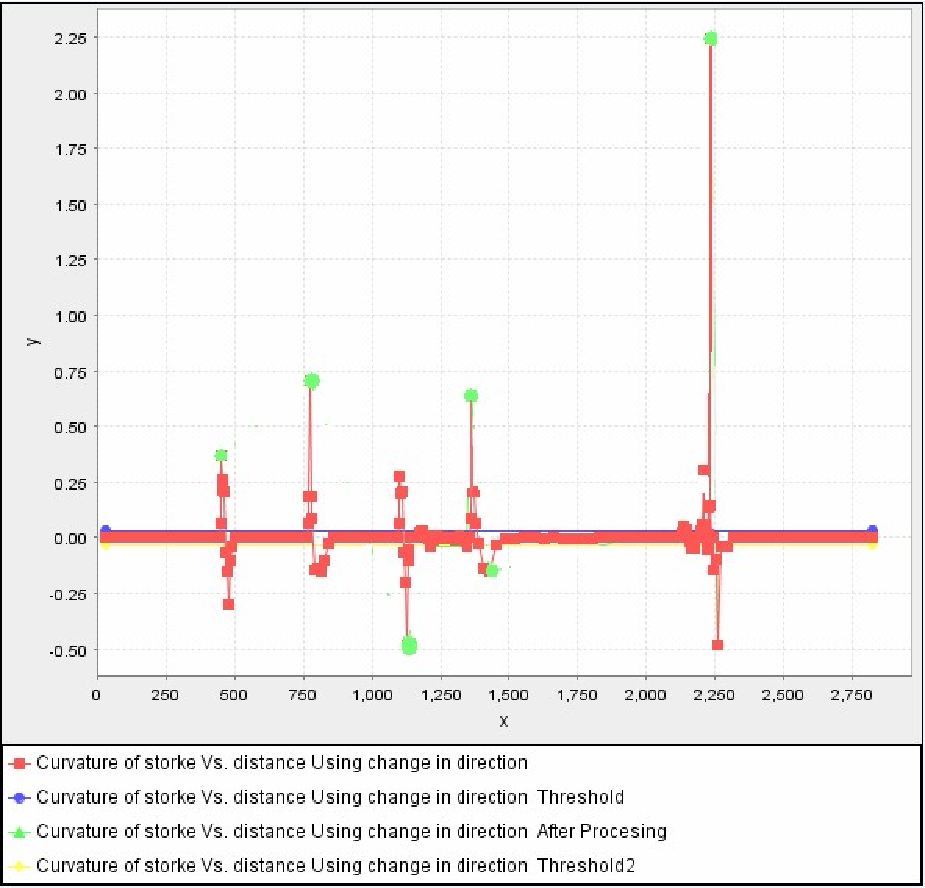
\includegraphics[scale=0.15]{images/curvature2.pdf}}
			
			\subfigure[ Time Difference] {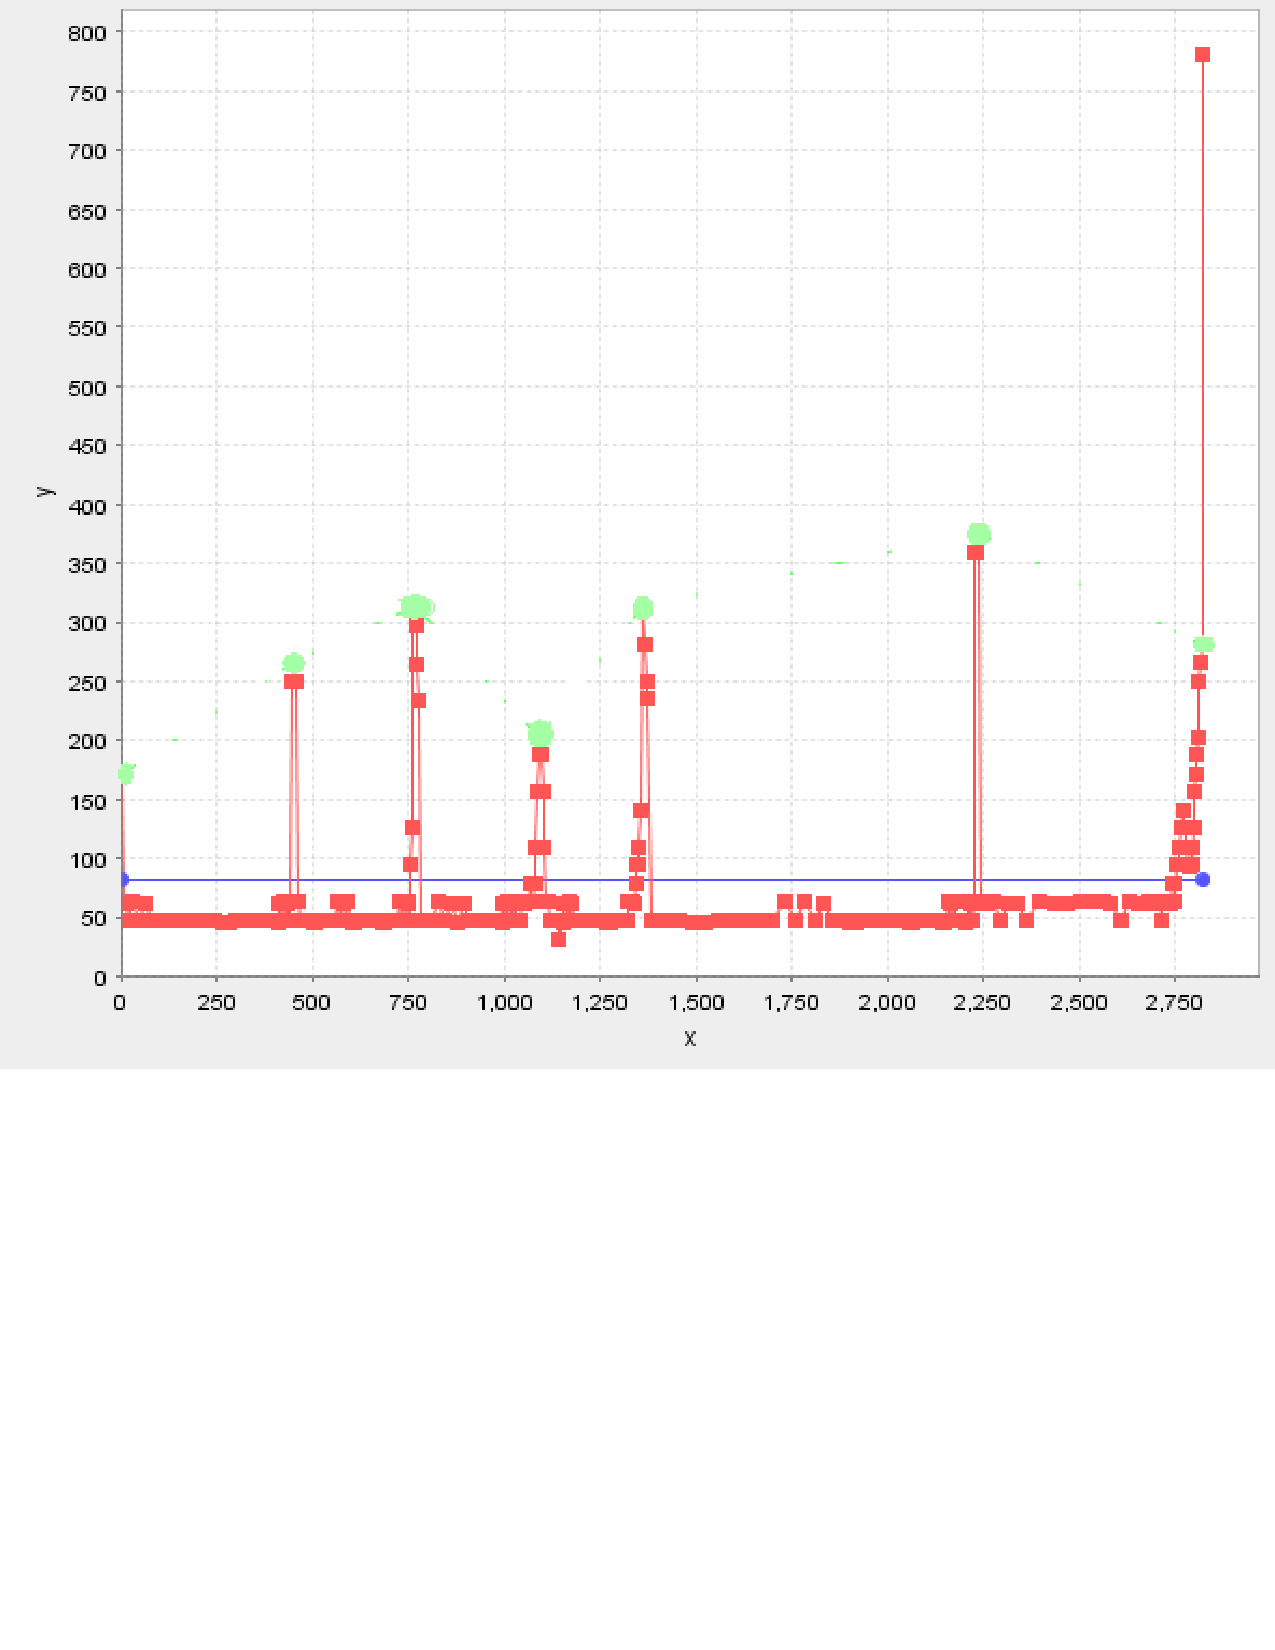
\includegraphics[scale=0.15]{images/time2.pdf}}
			\end{minipage}
	
	\caption[Data Curves]%{The data of the stroke}
	
	\label{fig:speed2}
\end{figure*}
%Description of input data. 
%how to calculate speed, curvature, area, bounding box.
%how to remove noise. 
%Finally how to compute primarily dominant points. 
\subsection{Segmentation}
\label{seg}
After computing the primary data the system now tries to segment the stroke into a set of primitives. The segmentation algorithm first tries to detect if the stroke is an ellipse. If the stroke proved to be an ellipse then the segmentation process ends and the system proceeds to the next step. Otherwise, the stroke is passed into two particle swarm algorithms that will divide the stroke to either lines or lines and curves. The algorithms takes the stroke points along with the possible dominant points computed then produce a set of dominant points which are connected with either lines or curves (see fig. \ref{fig:Blockdiagram}).  The next section will describe the ellipse detection algorithm and both the two particle swarm algorithms used to divide the stroke. \\
%Paragraphs describe the segmentation algorithm.  
\subsubsection{ Ellipse Detection } 
%Describe the ellipse detection algorithms 
The process starts with computing the center of the stroke bounding box. The bounding box center point is used as the first estimation of the center of the ellipse. The axes of the ellipse are estimated as the w/2 and h/2 of the stroke bounding box. The least square fitting algorithm is used to minimize the fitting error of the ellipse equation (see \ref{eq:circleFit} where N is number of points in the stroke, $a,b$ are the length of ellipse axes, $x_0$ \& $y_0$ are the coordinates of the center point, $x_i$ \& $y_i$ are the coordinates of point $i$ in the stroke). After only few loops the error and a confidence values  are computed to check if the storke can be labled as ellipse or not.\\ %is computed to check if stroke is an ellipse. \\
%We found that if the confidante is above threshold then the probability of ellipse is highest otherwise the stroke is passed to the next section to get the divisions of stroke and test its error.  
\begin{equation}
E = \sum\limits_{i = 0}^N {\frac{{(x_i - x_0 )}}{{a^2 }}^2  + \frac{{(y_i - y_0 )}}{{b^2 }}^2  - 1} 
\label{eq:circleFit}
\end{equation}
\subsubsection{ Discrete particle swarm algorithm}
There are two PSO algorithm described in this section. The system generates segmentation from both algorithms and then chooses the segmentation with the minimum error value. The problem definition is the same in both algorithms but they differ in the method they compute fitness and error functions. %formation is nearly the same in both. 
\subsubsection{ problem definition}
The input stroke with N points can be represented by set $S = \left\{ {x_1 ,x_2  \ldots x_N } \right\}$ where $x_i$ is the location of the point $i$ . The swarm algorithms consist of M agents which are represented by the set 
$A  = \left\{ {P_i \left| {i = 1,2 \cdots M} \right.} \right\}$ where $P_i$ is a single solution particle from the solution space. Each particle decodes the problem with binary array with the same length N as the input stroke.  
% The particles of the swarm represent a single solution of the solution space. For this problem the, each particle %will give a different segmentation for the input stroke. Firstly, we will define the stroke with N points by the set %S where.  We define the arc %An array with the same length as the number of points of the strokes.
So the system will represent each particle $P_i$ by $P_i = \left\{ {p_{ij} \left| {j = 1,2 \cdots N} \right.} \right\}$ where $p_{ij}$ will have only two values 0 or 1 where $p_{ij}=1$ will mean that point $j$ is a dominant point. 
% a!402B!
%$A = \left\{ {p_i \left| {i = 1,2 \cdots N} \right.} \right\}$
% a!402A!
%\begin{equation}
%A = \left\{ {p_i \left| {i = 1,2 \cdots N} \right.} \right\}.
%\end{equation}
\subsubsection{The algorithm}
The fitness function and error calculation are different in each algorithm. For the first algorithm, 
let's define the arc $\widehat{x_ix_j}$ as the consecutive set of points from point $x_i,x_{i+1} \cdots,x_j$. The line
$\overline{x_i x_j} $ as the straight line connecting point $x_i$ to point $x_j$. The approximation error is computed by the equation \ref{eq:ErrorSwarm1}  where M is the number of dominant points in this solution.  The error $ e ( \widehat{x_ix_j},\overline{x_i x_j})$ is computed as the sum of squared perpendicular distance from every point along the arc $\widehat{x_ix_j}$ to the line $\overline{x_i x_j}$.  \\
\begin{equation}
E=\sum\nolimits_{i = 0}^M e ( \widehat{x_ix_{i+1}},\overline{x_i x_{i+1}})
\label{eq:ErrorSwarm1}
\end{equation}
\begin{equation}
\max fitness(p_i ) = \left\{ {\begin{array}{*{20}c}
   { - E/\varepsilon N} & {ifE > \varepsilon ,}  \\
   {D/\sum\limits_{j = 1}^N {p_{ij} } } & {otherwise}  \\
\end{array}} \right.
\label{eq:fitnessSwarm1}
\end{equation}%\]
The fitness is computed using equation \ref{eq:fitnessSwarm1} where N is the number of points in the stroke, D is the number of point in the solution that was previously labeled as a possible dominant point and E is the computed error and $\varepsilon$ is the error threshold.   As you can see when the error is larger than the threshold is given a -ve value to lower the value of solution otherwise the system will favor the lower number of vertices.\\ %we will want to lower the number of vertices. \\
%if we say that s
%Alg1:
%Alg2: 
The second algorithm has the same problem formulation but different fitness and error functions. It was previously introduced in  \cite{CruveDivisionSwarm} where but genetic programming was used as the optimizing algorithm.  The error of both circle and line estimation are computed for each segment, the approximation with the lower error value will be the chosen approximation of this segment. The sum of the approximation error of all segments is the total error of the particle.  The error is computed by equation \ref{eq:errorSwarm2} where M is the number of segments in the solution, $D_i$ is the minimum approximation error of curve and line approximations $min(d_c,d_l)$ as computed by \cite{CruveDivisionSwarm}.  The fitness is computed by the equation \ref{eq:fitnessSwarm2} where E is the error and M is number of segments and k is a parameter tweaked to get minimum number of segments. \\
\begin{equation}
E=\sum\nolimits_{i = 0}^M e(D_i) 
\label{eq:errorSwarm2}
\end{equation}
\begin{equation}
\max fitness(P_i ) = \frac{1}{{E \times M^k }}
\label{eq:fitnessSwarm2}
\end{equation}
%Describe how we used particle swarm in curve polygon approximation using first algorithm.  
%Describe how we used PSO in to divide stroke into segments and curves. 
%[These two algorithm was modified from the algorithm in paper \cite{PolygonApproximationPSO,CruveDivisionSwarm}].
\cite{PolygonApproximationPSO} used a merge and divide algorithm after each loop of the swarm system to refine the solution but we used another enhancement method. After each loop in the swarm algorithm, each particle loops on the set of selected dominant points to enhance the solution. Each dominant point is checked to find if it was labeled before as a possible dominant (computed as in section \ref{Prepross}), if not the point is moved to the nearest labeled point.    
%check the new solution and check the new vertices if a vertex points is a possible dominant point it is left as a vertex. Otherwise, the system will search in the local neighborhood for the nearest possible dominant point to move these vertices to. After each change the error is computed and if new error is less that the old then the new set is approved. \\
\subsection{Recognition}
After the user draw all strokes of the symbol he has to wait 10 seconds or press finish button beside the drawing area. The set of unrecognized strokes is grouped together along with their segmentation as input to the feature extraction process. The system uses a composite set of features include Rubine feature set \cite{gestureexample12}, Zernike moments \cite{HeloiseBeautification}, ink density \cite{GeometryAndDomain102} and some structural information like number of perpendiculars lines , number of parallel lines and types of primitives in each symbol. After computing the features the symbol is introduced to the classifier. The system used a support vector machine (SVM) classifier with Gaussian kernel (RBF kernel) \cite{libsvm}.\\%Some features like number of parallel, perpendicular and intersecting lines are computed from the segmentation other like density, centroid and Zernike moments are computed from the raw stroke points. 
 %trained with the 13 categories in the system. The same training set was used by \cite{HeloiseBeautification} in their symbol recognition system. \\ %  The table describe the features used in the system. 
%\begin{table}
%\begin{minipage}[t][1\totalheight]{0.3\columnwidth}
%
%\begin{tabular}{|l|l|l|}
%\hline 
%Type & Features & Notes\tabularnewline
%\hline 
%\hline Structural & No. of parallel lines & \tabularnewline
%\hline & No. of perpendicular lines & \tabularnewline
%\hline & No. of intersections & \tabularnewline
%\hline Statistical & Mean and standard deviation of the Curvature data   & \tabularnewline
%\hline & Mean of the speed data & \tabularnewline
%\hline 
%Rubine & Set of features \\for gesture recognition & Introduced by Rubine in \cite{} \tabularnewline
%\hline Zernike &  A Zernike\\ moments  &  Used by \cite{zernike61} \tabularnewline
%\hline Composite & width to\\ height ratio  & \tabularnewline
%\hline  & ink density  & Used by \cite{} \tabularnewline
%\hline
%\end{tabular}		
%\end{minipage}
%	\caption{Feature Table}
%	\label{tab:FeatureTable}
%\end{table}
  % Rubine el al.\cite{gestureexample12}  used a set of statistical features,  There are a lot of features used in the sketch recognition literature
%How to handle multi-stroked symbols. 
%The clustering algorithm.  
%The classifier used in recognition
%Describe the features used in recognition [ref to \cite{zernike61}]
\section{Experiments}\label{sec:Experiments}
For testing the system used a data set collected by \citeauthor{HeloiseBeautification}. The data are drawn by 16 users each of them have drawn from 30 to 50 samples for each shape. Figure \ref{fig:symbolSet} shows the shapes used in the data set. We divided the dataset equally into training set and test set.  The results displayed are the recognition accuracy resulted from the classifier after recognizing the symbols. \\
%We divided the dataset into four sets each set contains four different users. Furthermore, each set is divided into train and test set where the trained set where used to train the classifiers and the test set where used for testing.  The algorithms are then tested using the four sets and the results are averaged.
\begin{figure}[]\centering
\fbox{  \parbox{4cm}{% 
		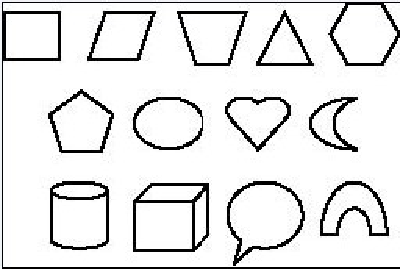
\includegraphics[scale=0.4]{images/symbolSet.pdf}	}}
	\caption{The Symbol Set}
	\label{fig:symbolSet}
\end{figure}
\begin{figure}[]
	\centering
		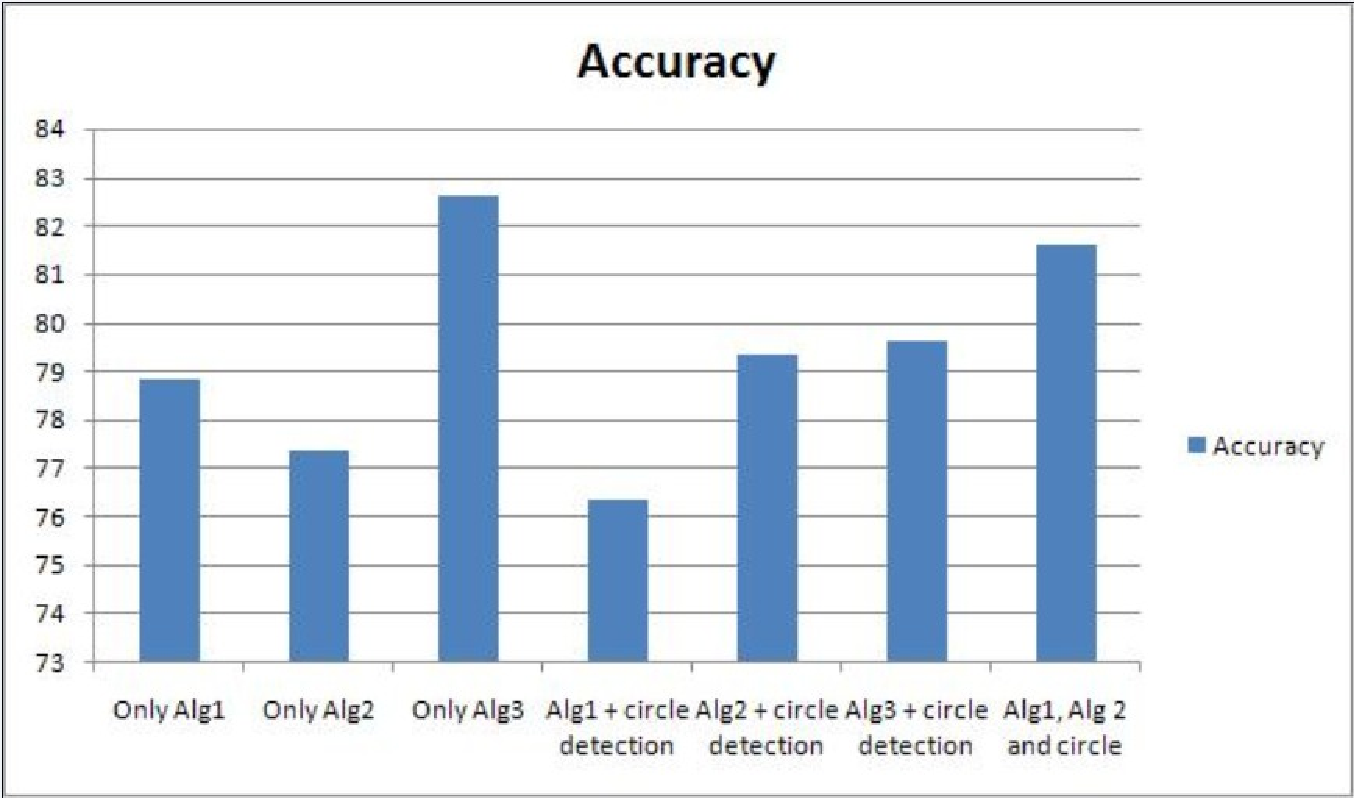
\includegraphics[scale=0.3]{images/test1.pdf}
	\caption{The results of first experiment}
	\label{fig:test1}
\end{figure}
%In the figure \ref{fig:test1}, the accuracy means that final hit rate of all symbols used in the test set.by the  four datasets . 
We performed three experiments to test the system firstly we tested recognition accuracy of shapes in the data set with both algorithms. We also implemented the segmentation algorithm described in \cite{earlyprocess} to use as reference to our swarm algorithms.  As you see in the fig. \ref{fig:test1} shows the accuracy achieved by each algorithm. The results shows that both PSO algorithm achieve better result than other algorithms.  The swarm algorithms were tested with and without the ellipse detection module. The ellipse detection module appear to be superior to results with only the PSO algorithms.  \\  

The second experiment we implemented was to test the effect of symbol complexity and type on the recognition rate. Figure \ref{fig:test2} shows what the accuracy of each symbol, it clearly noted that symbols that have only line segments achieve higher accuracy rate than other symbols. Figure \ref{fig:test2} also shows that algorithm 1 alone achieve better performance than algorithm 2 in the symbols that consist of lines only. The combining of both algorithm improves the recognition rate of other symbols.  \\
\begin{figure*}[]
	\centering
		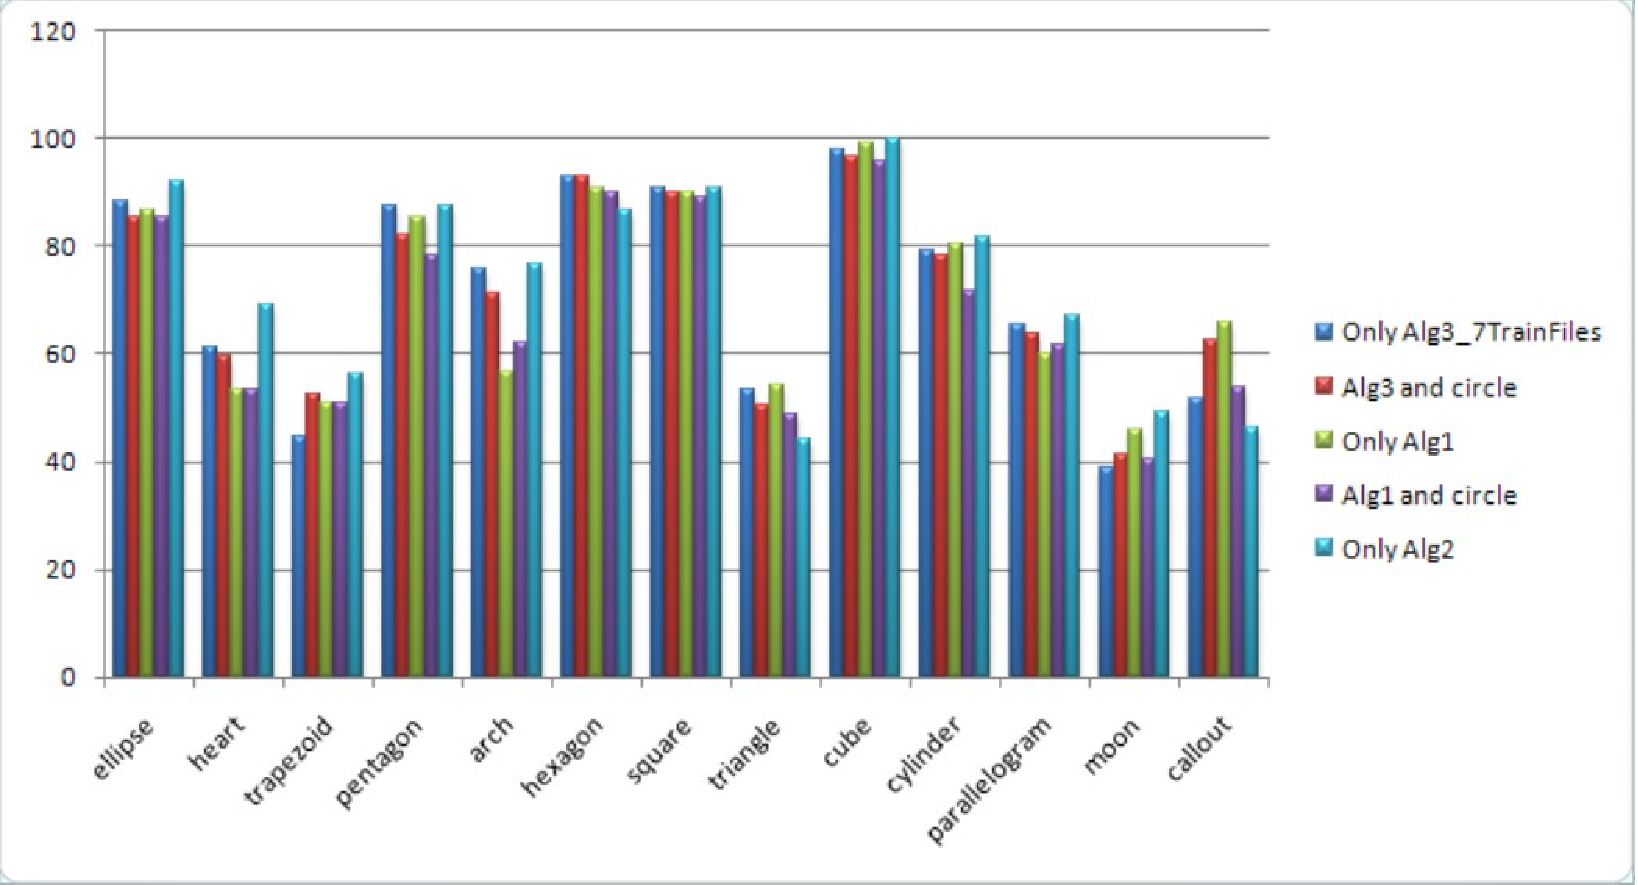
\includegraphics[scale=0.5]{images/test2.pdf}
	\caption{The results of second experiment}
	\label{fig:test2}
\end{figure*}
  The final experiment we performed was to test the efficiency svm classifier. We implemented the linear discriminator classifier described in \cite{gestureexample12}(see figure \ref{fig:test3}).  %The result shows that SVM is more scalable than the linear discriminator for this problem. %The test focus on the size of data needed to test each classifier and the achieved accuracy.  %For this experiment we also shows the classification time for both classifiers 
\begin{figure}[]
	\centering
		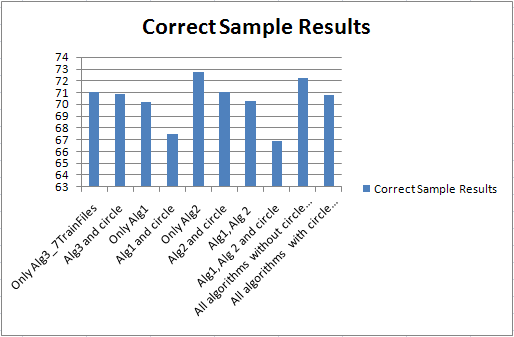
\includegraphics[scale=0.4]{images/test1.png}
	\caption{The results of third experiment}
	\label{fig:test3}
\end{figure}
 %Details description of results got from comparing various algorithms  
 %Describe data set used for experiments ( No of data set, No. of categories, No of samples).
 %Describe other Algorithms [Alg 3 in paper \cite{earlyprocess}]used for comparing with the one described in the paper. 
\section{Conclusion}
This paper presented a new approach to sketch recognition using PSO. It was noted that the PSO in general improve the accuracy of the final symbol recognition in the system. The use of both speed and curvature data helps in improvement of the PSO algorithm over the original algorithms \cite{CruveDivisionSwarm,PolygonApproximationPSO}. The tradeoff between accuracy achieved and time complexity must be further investigated to achieve better results.  
%As you can see form the experiments PSO have proved a spuriously than other system. 
\section{Future Work}
The next step in this research is to complete the clustering algorithm for fully automated sketch recognition. The clustering must be performed without the user explicit involvement. Other area of modification can be the features extraction and classifier. Adding more spatial features will improve classifications.  %Each new stroke is checked if it can be a symbol or is a part of already drawn un completed symbol. 
%\bibliography{Mybibliography}
\bibliography{../../neededfiles/Bibliographies/Mybibliography2}
\end{document}
